% Created 2012-10-17 Wed 13:52
\documentclass[11pt]{article}
\usepackage[utf8]{inputenc}
\usepackage{fixltx2e}
\usepackage{url}
\usepackage{graphicx}
\usepackage{minted}
\usepackage{color}
\usepackage{longtable}
\usepackage{float}
\usepackage{wrapfig}
\usepackage{soul}
\usepackage{textcomp}
\usepackage{amsmath}
\usepackage{marvosym}
\usepackage{wasysym}
\usepackage{latexsym}
\usepackage{amssymb}
\usepackage[linktocpage,
  pdfstartview=FitH,
  colorlinks,
  linkcolor=blue,
  anchorcolor=blue,
  citecolor=blue,
  filecolor=blue,
  menucolor=blue,
  urlcolor=blue]{hyperref}
\usepackage{attachfile}
\tolerance=1000
\usepackage{adjustbox}
\usepackage{anysize}
\marginsize{1in}{1in}{1in}{1in}
\providecommand{\alert}[1]{\textbf{#1}}

\title{Molecular Simulation HOMEWORK 4}
\author{Zhongnan Xu}
\date{10/24/12 - Wednesday}
\hypersetup{
  pdfkeywords={},
  pdfsubject={},
  pdfcreator={Emacs Org-mode version 7.8.11}}

\begin{document}

\maketitle

\setcounter{tocdepth}{3}
\tableofcontents
\vspace*{1cm}


\section{Convergence study of tantalum}
\label{sec-1}
\subsection{Planewave cutoff convergence}
\label{sec-1-1}

Determine the planewave cutoff energy required to achieve a total energy convergence of 10 meV for bcc tantalum at its experimental lattice constant. Use a k-point grid of 10 \texttimes{} 10 \texttimes{} 10, and the PBE exchange correlation functional.


\begin{minted}[frame=lines,fontsize=\scriptsize,linenos]{python}
from ase import Atom, Atoms
from ase.visualize import view
import numpy as np
import matplotlib.pyplot as plt
from jasp import *
ready=True
a = 3.31 # Taken from Lange's Handbook of Chemistry 
a1 = np.array((-a/2, a/2, a/2))
a2 = np.array((a/2, -a/2, a/2))
a3 = np.array((a/2, a/2, -a/2))
Ta = Atoms([Atom('Ta', (0, 0, 0), magmom=6)],
           cell=(a1, a2, a3))
encuts = (150, 200, 250, 300, 350, 400, 450, 500)
energies = []
for cut in encuts:
    with jasp('1.1/e{0:d}'.format(cut),
              xc='PBE', lreal=False, istart=0,
              encut=cut, prec='Accurate',
              kpts=(10, 10, 10), ismear=1, sigma=0.05,
              ispin=2, lorbit=11,
              atoms=Ta) as calc:
        try:
            energies.append(Ta.get_potential_energy())
        except (VaspSubmitted, VaspQueued):
            energies.append(None)
            ready = False
            pass
assert len(encuts) == len(energies)
if not ready:
    import sys; sys.exit()

import matplotlib.pyplot as plt
from matplotlib.ticker import ScalarFormatter
# First offset the energies by the last value and find the absolute value
energies = np.array(energies)
energies -= energies[-1]*np.ones(len(energies))
energies = np.absolute(energies)
energies = energies*1000
fig = plt.figure(1, (5.5, 4.5))
ax = fig.add_subplot(111)
ax.plot(encuts, energies, label='Ta', marker='o')
ax.axhline(10, ls='--', label='10 meV Convergence')
ax.set_xlabel('Kinetic Energy Cutoff (eV)', size='large')
ax.set_ylabel('Total Energy (meV/atom)', size='large')
ax.legend(loc=0, prop={'size':'large'})
ax.yaxis.set_major_formatter(ScalarFormatter(useOffset=False))
fig.tight_layout()
plt.savefig('1-1.png')
plt.show()
\end{minted}


\begin{figure}[H]
\centering
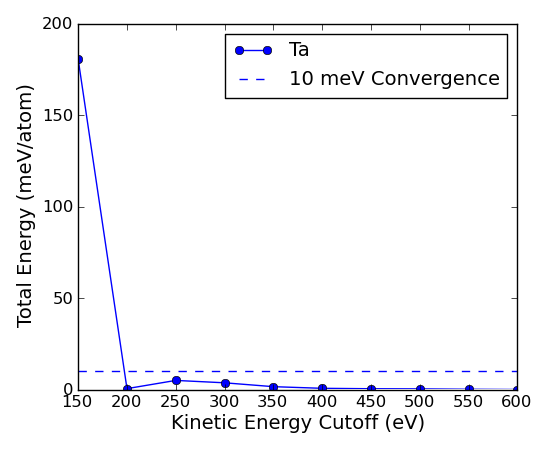
\includegraphics[width=0.7\textwidth]{./1-1.png}
\caption{Convergence of the total energy of BCC Ta at the experimental lattice cutoff}
\end{figure}

It is clear that the total energy of BCC Ta has already been converged at an energy cutoff of 200 eV. This should not be surprising considering the VASP site recommends a minimum cutoff of 220 eV.
\subsection{k-point grid convergence}
\label{sec-1-2}

Determine the Monkhorst-Pack k-point grid required to achieve a total energy convergence of 50 meV for bcc tantalum at its experimental lattice constant. Use a planewave cutoff of 350 eV for this study.


\begin{minted}[frame=lines,fontsize=\scriptsize,linenos]{python}
from ase import Atom, Atoms
from ase.visualize import view
from ase.lattice.cubic import BodyCenteredCubic
import numpy as np
import matplotlib.pyplot as plt
from jasp import *

# We will rely on the ase.lattice.cubic.BodyCenteredCubic module to give us
# the correct experimental lattice constant. Note we use the primitive cell
ready=True
a = 3.31
a1 = np.array((-a/2, a/2, a/2))
a2 = np.array((a/2, -a/2, a/2))
a3 = np.array((a/2, a/2, -a/2))
Ta = Atoms([Atom('Ta', (0, 0, 0), magmom=6)],
           cell=(a1, a2, a3))

ks = (2, 4, 6, 8, 10, 12, 14, 16)
kpoints = []
for k in ks:
    kpoints.append((k, k, k))
energies = []
for kpoint in kpoints:
    with jasp('1.2/k{0:d}'.format(kpoint[0]),
              xc='PBE', lreal=False, istart=0,
              encut=350, prec='Accurate',
              kpts=kpoint, ismear=1, sigma=0.05,
              ispin=2, lorbit=11,
              atoms=Ta) as calc:
        try:
            energies.append(Ta.get_potential_energy())
        except (VaspSubmitted, VaspQueued):
            energies.append(None)
            ready = False
            pass
assert len(ks) == len(energies)
if not ready:
    import sys; sys.exit()

import matplotlib.pyplot as plt
from matplotlib.ticker import ScalarFormatter
# First offset the energies by the last value and find the absolute value
energies = np.array(energies)
energies -= energies[-1]*np.ones(len(energies))
energies = np.absolute(energies)
energies = energies*1000
fig = plt.figure(1, (5.5, 4.5))
ax = fig.add_subplot(111)
ax.plot(ks, energies, label='Ta', marker='o')
ax.axhline(50, ls='--', label='50 meV convergence')
ax.set_ylim((0, 100))
ax.set_xlabel(r'Kpoint Grid (N$\times$ N$\times$ N)', size='large')
ax.set_ylabel('Total Energy (meV/atom)', size='large')
ax.legend(loc=0, prop={'size':'large'})
ax.yaxis.set_major_formatter(ScalarFormatter(useOffset=False))
fig.tight_layout()
plt.savefig('1-2.png')
plt.show()
\end{minted}


\begin{figure}[H]
\centering
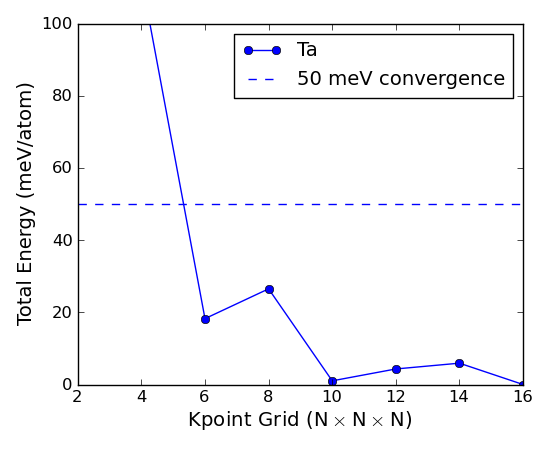
\includegraphics[width=0.7\textwidth]{./1-2.png}
\caption{Convergence of BCC Ta with respect to increasing k-point grid}
\end{figure}
BCC Ta is converged within 50 meV by a k-point grid size of 6 \texttimes{} 6 \texttimes{} 6.
\section{Convergence study of graphite}
\label{sec-2}
\subsection{Planewave convergence}
\label{sec-2-1}

Determine the planewave cutoff energy required to get convergence of 10 meV or better for graphite at its equilibrium lattice constant. Use a k-point grid of (6,6,6) for this study.


\begin{minted}[frame=lines,fontsize=\scriptsize,linenos]{python}
from jasp import *
from ase.lattice.hexagonal import Graphite
from ase.visualize import view

ready = True

atoms = Graphite('C', latticeconstant={'a':2.4612, 'c':6.7079})
encuts = (250, 300, 350, 400, 450, 500)
energies = []
for cut in encuts:
    with jasp('2.1/e{0:d}'.format(cut),
              xc='PBE', lreal=False, istart=0,
              encut=cut, prec='Accurate',
              kpts=(6, 6, 6), ismear=1, sigma=0.05, gamma=True,
              ispin=2, lorbit=11,
              atoms=atoms) as calc:
        try:
            energies.append(atoms.get_potential_energy())
        except (VaspSubmitted, VaspQueued):
            energies.append(None)
            ready = False
            pass
assert len(encuts) == len(energies)
if not ready:
    import sys; sys.exit()

import matplotlib.pyplot as plt
from matplotlib.ticker import ScalarFormatter
# First offset the energies by the last value and find the absolute value
energies = np.array(energies)
energies -= energies[-1]*np.ones(len(energies))
energies = np.absolute(energies)
energies = energies*1000
fig = plt.figure(1, (5.5, 4.5))
ax = fig.add_subplot(111)
ax.plot(encuts, energies, label='Graphite', marker='o')
ax.axhline(10, ls='--', label='10 meV Convergence')
ax.set_xlabel('Kinetic Energy Cutoff (eV)', size='large')
ax.set_ylabel('Total Energy (meV/atom)', size='large')
ax.legend(loc=0, prop={'size':'large'})
ax.yaxis.set_major_formatter(ScalarFormatter(useOffset=False))
fig.tight_layout()
plt.savefig('2-1.png')
plt.show()
\end{minted}


\begin{figure}[H]
\centering
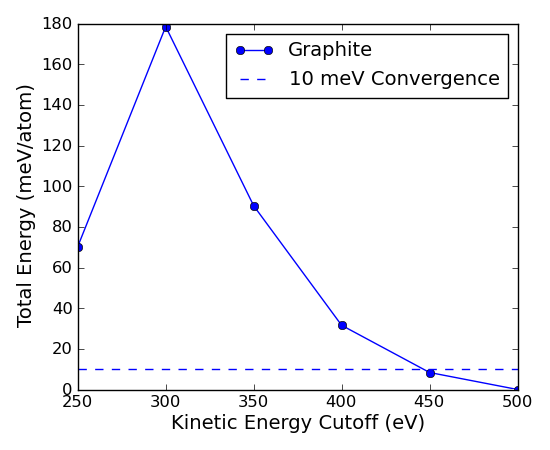
\includegraphics[width=0.7\textwidth]{./2-1.png}
\caption{Convergence of graphite with respect to increasing kinetic energy cutoff}
\end{figure}

Graphite converges within 450 eV plane wave cutoff energy.
\subsection{k-point convergence}
\label{sec-2-2}

   Determine the k-point grid required to get convergence of 50 meV or better for graphite at its equilibrium lattice constant. Use a planewave cutoff of 350 eV for this study.

Note, I used a gamma point grid spacing because we are using a hexagonal cell. The VASP site recommends the use of gamma point spacing for hexagonal unit cells.


\begin{minted}[frame=lines,fontsize=\scriptsize,linenos]{python}
from jasp import *
from ase.lattice.hexagonal import Graphite

# We will rely on the ase.lattice.cubic.BodyCenteredCubic module to give us
# the correct experimental lattice constant. Note we use the primitive cell
ready=True

atoms = Graphite('C', latticeconstant={'a':2.4612, 'c':6.7079})
ks = (2, 4, 6, 8, 10, 12, 14, 16)
kpoints = []
for k in ks:
    kpoints.append((k, k, k))
energies = []
for kpoint in kpoints:
    with jasp('2.2/k{0:d}'.format(kpoint[0]),
              xc='PBE', lreal=False,
              encut=350, prec='Accurate',
              kpts=kpoint, ismear=1, sigma=0.05, gamma=True,
              ispin=2, lorbit=11,
              atoms=atoms) as calc:
        try:
            energies.append(atoms.get_potential_energy())
        except (VaspSubmitted, VaspQueued):
            energies.append(None)
            ready = False
            pass
assert len(ks) == len(energies)
if not ready:
    import sys; sys.exit()

import matplotlib.pyplot as plt
from matplotlib.ticker import ScalarFormatter
# First offset the energies by the last value and find the absolute value
energies = np.array(energies)
energies -= energies[-1]*np.ones(len(energies))
energies = np.absolute(energies)
energies = energies*1000
fig = plt.figure(1, (5.5, 4.5))
ax = fig.add_subplot(111)
ax.plot(ks, energies, label='Graphite', marker='o')
ax.axhline(50, ls='--', label='50 meV convergence')
ax.set_ylim((0, 100))
ax.set_xlabel(r'Kpoint Grid (N$\times$ N$\times$ N)', size='large')
ax.set_ylabel('Total Energy (meV/atom)', size='large')
ax.legend(loc=0, prop={'size':'large'})
ax.yaxis.set_major_formatter(ScalarFormatter(useOffset=False))
fig.tight_layout()
plt.savefig('2-2.png')
plt.show()
\end{minted}

\begin{figure}[H]
\centering
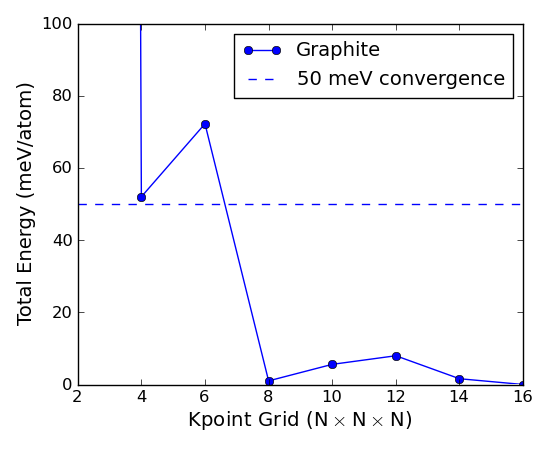
\includegraphics[width=0.7\textwidth]{./2-2.png}
\caption{Convergence of Graphite with respect to increasing k-point grid}
\end{figure}

Graphite converges within an 8 \texttimes{} 8 \texttimes{} 8 kpoint gamma point grid spacing.
\section{Determine the DFT lattice constant of bcc tantalum}
\label{sec-3}

  Use the parameters you estimated in the previous problem. Construct an equation of state and determine the lattice constant and bulk modulus of tantalum. Compare your answers to literature values, and cite the source of your comparison.


\begin{minted}[frame=lines,fontsize=\scriptsize,linenos]{python}
from jasp import *
from ase.lattice.cubic import BodyCenteredCubic
import numpy as np
import matplotlib.pyplot as plt

ready=True
lat = 3.31 # Taken from Lange's Handbook of Chemistry 
space = 0.02
lats = (lat - 2*space,
        lat - space,
        lat,
        lat + space,
        lat + 2*space)
energies, volumes  = [], []
for a in lats:
    a1 = np.array((-a/2, a/2, a/2))
    a2 = np.array((a/2, -a/2, a/2))
    a3 = np.array((a/2, a/2, -a/2))
    Ta = Atoms([Atom('Ta', (0, 0, 0), magmom=6)],
               cell=(a1, a2, a3))
    with jasp('3.1/a-{0:1.2f}'.format(a),
              xc='PBE', lreal=False, istart=0,
              encut=200, prec='Accurate',
              kpts=(6, 6, 6), ismear=1, sigma=0.05,
              ispin=2, lorbit=11,
              atoms=Ta) as calc:
        try:
            energies.append(Ta.get_potential_energy())
            volumes.append(Ta.get_volume())
        except (VaspSubmitted, VaspQueued):
            energies.append(None)
            ready = False
            pass
if not ready:
    import sys; sys.exit()

from ase.utils.eos import EquationOfState
eos = EquationOfState(volumes, energies)
v0, e0, B = eos.fit()
eqlat = (2*v0) ** (1./3.)
print 'The equilibrium lattice constant is {0:1.3f} Angstroms'.format(eqlat)
print 'The bulk modulus is {0:1.3f} eV/Angstroms^3'.format(B)
eos.plot('3-1.png')
\end{minted}

\begin{verbatim}
 The equilibrium lattice constant is 3.305 Angstroms
 The bulk modulus is 1.323 eV/Angstroms^3
\end{verbatim}

\begin{figure}[H]
\centering
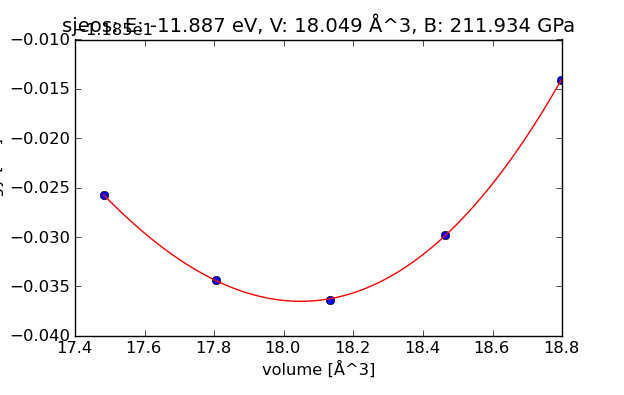
\includegraphics[width=0.7\textwidth]{./3-1.png}
\caption{Convergence of Graphite with respect to increasing k-point grid}
\end{figure}
\section{Determine the DFT lattice constant of fcc tantalum}
\label{sec-4}

Construct an equation of state to determine the lattice constant of fcc tantalum. You can assume the same parameters that were good for the bcc structure are good for the fcc structure. Which structure is more stable, fcc or bcc?
\bigskipt

First we have to calculate the lattice constant of an FCC structure that corresponds to around 3.31 \AA{} lattice constant of the BCC structure

The volume of the FCC primitive cell in terms of the lattice constant is $V_{\mathrm{fcc}} = \frac{a_{\mathrm{fcc}}^3}{4}$ while that of the BCC primitive cell is $V_{\mathrm{bcc}} = \frac{a_{\mathrm{bcc}}^3}{2}$. Setting these two equal, we see that $a_{\mathrm{fcc}} = (2a_{\mathrm{bcc}}^{3})^{1/3}$. 


\begin{minted}[frame=lines,fontsize=\scriptsize,linenos]{python}
a_fcc = (2*3.31**3)**(1./3.)
print 'A good guess for the FCC lattice constant is {0:1.3f}'.format(a_fcc)
\end{minted}

\begin{verbatim}
 A good guess for the FCC lattice constant is 4.170
\end{verbatim}

Now we can compute the EOS for FCC Ta.


\begin{minted}[frame=lines,fontsize=\scriptsize,linenos]{python}
from jasp import *
import numpy as np
import matplotlib.pyplot as plt

ready=True
lat = 4.170
space = 0.02
lats = (lat - 2*space,
        lat - space,
        lat,
        lat + space,
        lat + 2*space,
        lat + 3*space,
        lat + 4*space,
        lat + 5*space)
energies, volumes  = [], []
for a in lats:
    a1 = np.array((0, a/2, a/2))
    a2 = np.array((a/2, 0, a/2))
    a3 = np.array((a/2, a/2, 0))
    Ta = Atoms([Atom('Ta', (0, 0, 0), magmom=6)],
               cell=(a1, a2, a3))
    with jasp('4.1/a-{0:1.2f}'.format(a),
              xc='PBE', lreal=False, istart=0,
              encut=200, prec='Accurate',
              kpts=(6, 6, 6), ismear=1, sigma=0.05,
              ispin=2, lorbit=11,
              atoms=Ta) as calc:
        try:
            energies.append(Ta.get_potential_energy())
            volumes.append(Ta.get_volume())
        except (VaspSubmitted, VaspQueued):
            energies.append(None)
            ready = False
            pass
if not ready:
    import sys; sys.exit()

from ase.utils.eos import EquationOfState
eos = EquationOfState(volumes, energies)
v0, e0, B = eos.fit()
eqlat = (4*v0) ** (1./3.)
print 'The equilibrium lattice constant is {0:1.3f} Angstroms'.format(eqlat)
print 'The bulk modulus is {0:1.3f} eV/Angstroms^3'.format(B)
eos.plot('4-1.png')
\end{minted}

\begin{verbatim}
 The equilibrium lattice constant is 4.214 Angstroms
 The bulk modulus is 1.222 eV/Angstroms^3
\end{verbatim}

\begin{figure}[H]
\centering
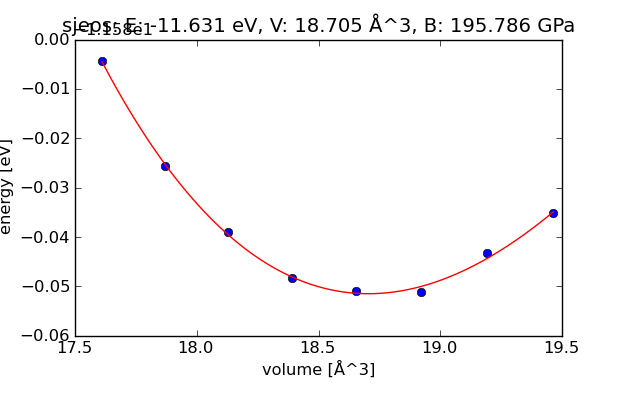
\includegraphics[width=0.7\textwidth]{./4-1.png}
\caption{Equation of state for FCC tantalum}
\end{figure}

According the equation of state, we have a minimum at 4.214 \AA{}. However, the equation of state clearly shows a volume with a lower energy than the minimum. Furthermore, the points are not smoothly fitted to a line, which suggests that the energies are not converged. From my experience, increasing the k-point spacing or kinetic energy cutoff will give us a smoother EOS. Lets do both.


\begin{minted}[frame=lines,fontsize=\scriptsize,linenos]{python}
from jasp import *
import numpy as np
import matplotlib.pyplot as plt

ready=True
lat = 4.170
space = 0.02
lats = (lat - 2*space,
        lat - space,
        lat,
        lat + space,
        lat + 2*space,
        lat + 3*space,
        lat + 4*space,
        lat + 5*space)
energies, volumes  = [], []
for a in lats:
    a1 = np.array((0, a/2, a/2))
    a2 = np.array((a/2, 0, a/2))
    a3 = np.array((a/2, a/2, 0))
    Ta = Atoms([Atom('Ta', (0, 0, 0), magmom=6)],
               cell=(a1, a2, a3))
    with jasp('4.2/a-{0:1.2f}'.format(a),
              xc='PBE', lreal=False, istart=0,
              encut=400, prec='Accurate',
              kpts=(8, 8, 8), ismear=1, sigma=0.05,
              ispin=2, lorbit=11,
              atoms=Ta) as calc:
        try:
            energies.append(Ta.get_potential_energy())
            volumes.append(Ta.get_volume())
        except (VaspSubmitted, VaspQueued):
            energies.append(None)
            ready = False
            pass
if not ready:
    import sys; sys.exit()

from ase.utils.eos import EquationOfState
eos = EquationOfState(volumes, energies)
v0, e0, B = eos.fit()
eqlat = (4*v0) ** (1./3.)
print 'The equilibrium lattice constant is {0:1.3f} Angstroms'.format(eqlat)
print 'The bulk modulus is {0:1.3f} eV/Angstroms^3'.format(B)
eos.plot('4-2.png')
\end{minted}

\begin{verbatim}
 The equilibrium lattice constant is 4.208 Angstroms
 The bulk modulus is 1.254 eV/Angstroms^3
\end{verbatim}

\begin{figure}[H]
\centering
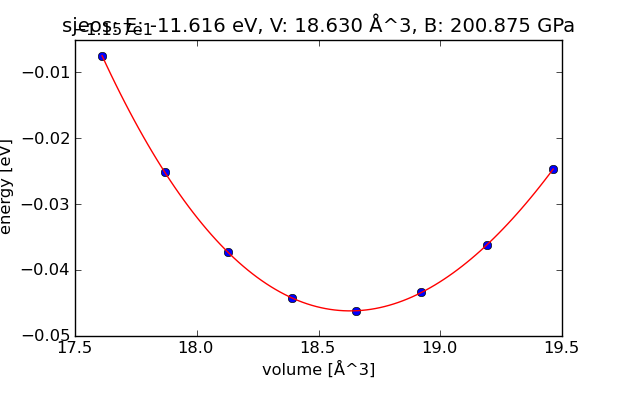
\includegraphics[width=0.7\textwidth]{./4-2.png}
\caption{Convergence of Graphite with respect to increasing k-point grid}
\end{figure}

We see that the higher parameters smoothed out the EOS and gives us an equilibriuim lattice constant of 4.208 \AA{} for Ta FCC. Now lets plot both graphs and look at their relative energetics.


\begin{minted}[frame=lines,fontsize=\scriptsize,linenos]{python}
from jasp import *
import numpy as np
import matplotlib.pyplot as plt

lat = 3.31
space = 0.02
lats = (lat - 2*space,
        lat - space,
        lat,
        lat + space,
        lat + 2*space)
bcc_energies, bcc_volumes  = [], []
for a in lats:
    a1 = np.array((-a/2, a/2, a/2))
    a2 = np.array((a/2, -a/2, a/2))
    a3 = np.array((a/2, a/2, -a/2))
    Ta = Atoms([Atom('Ta', (0, 0, 0), magmom=6)],
               cell=(a1, a2, a3))
    with jasp('3.1/a-{0:1.2f}'.format(a), atoms=Ta) as calc:
        bcc_energies.append(Ta.get_potential_energy())
        bcc_volumes.append(Ta.get_volume())

lat = 4.170
space = 0.02
lats = (lat - 2*space,
        lat - space,
        lat,
        lat + space,
        lat + 2*space,
        lat + 3*space,
        lat + 4*space,
        lat + 5*space)
fcc_energies, fcc_volumes  = [], []
for a in lats:
    a1 = np.array((0, a/2, a/2))
    a2 = np.array((a/2, 0, a/2))
    a3 = np.array((a/2, a/2, 0))
    Ta = Atoms([Atom('Ta', (0, 0, 0), magmom=6)],
               cell=(a1, a2, a3))
    with jasp('4.2/a-{0:1.2f}'.format(a), atoms=Ta) as calc:
        fcc_energies.append(Ta.get_potential_energy())
        fcc_volumes.append(Ta.get_volume())

fig = plt.figure(1, (5.5, 4.5))
ax = fig.add_subplot(111)
ax.plot(bcc_volumes, bcc_energies, label='Ta-BCC')
ax.plot(fcc_volumes, fcc_energies, label='Ta-FCC')
ax.legend(loc=0, prop={'size':'large'})
ax.set_xlabel('Volume per Ta atom', size='large')
ax.set_ylabel('Total energy per Ta atom (eV/atom)', size='large')
ax.ticklabel_format(useOffset=False)
fig.tight_layout()
plt.savefig('4-3.png')
plt.show()
\end{minted}


\begin{figure}[H]
\centering
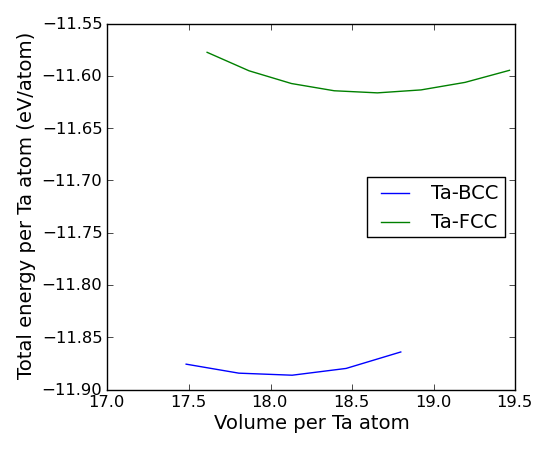
\includegraphics[width=0.7\textwidth]{./4-3.png}
\caption{Comparison between the FCC and BCC phases of Ta.}
\end{figure}

It is clear that the BCC phase of Ta is more stable than the FCC phase of Ta.
\section{Determine graphite lattice parameters}
\label{sec-5}

The crystal structure of graphite can be found at \href{http://cst-www.nrl.navy.mil/lattice/struk/a9.html}{http://cst-www.nrl.navy.mil/lattice/struk/a9.html} (or you can use the builtin \texttt{ase} functions).

Compute the geometry optimized total energy for graphite. Use parameters determined from the convergence study to ensure the total energy is converged to better than 50 meV. Compare your results to experimental data. Cite your source.


\begin{minted}[frame=lines,fontsize=\scriptsize,linenos]{python}
from jasp import *
from ase.lattice.hexagonal import Graphite
from ase.visualize import view

ready = True

graphite = Graphite('C', latticeconstant={'a':2.4612, 'c':6.7079})
with jasp('5.1/trial1', atoms=graphite,
          xc='PBE', lreal=False, istart=0,
          encut=450, prec='Accurate',
          kpts=(8, 8, 8), ismear=1, sigma=0.05, gamma=True,
          ibrion=1, isif=3, nsw=50, ediffg=-0.05, 
          ispin=2, lorbit=11) as calc:
    try:
        calc.calculate()
        new_cell = calc.get_atoms().cell
    except (VaspSubmitted, VaspQueued):
        ready = False
        pass
    print 'New Lattice Vectors'
    print '-------------------'
    print 'a1 = {0}'.format(new_cell[0])
    print 'a2 = {0}'.format(new_cell[1])
    print 'a3 = {0}'.format(new_cell[2])
\end{minted}

\begin{verbatim}
 New Lattice Vectors
 -------------------
 a1 = [ 2.466  0.     0.   ]
 a2 = [-1.233  2.136  0.   ]
 a3 = [ 0.     0.     7.075]
\end{verbatim}

From these results, we see the relaxed lattice parameters are a=2.466 and c=7.075. The experimental lattice parameter was shown to be a=2.4612 and c=6.7079 from the dft book and a review on graphite \footnote{D. Chung, Journal of Material Science 37, 1475 (2002).
 }. This is not surprising because DFT has been known to not be able to accurately describe Van Der Waals forces, which accounts for the bonding between the carbon layers in graphite.
\section{Tantalum carbide lattice parameters}
\label{sec-6}

Tantalum carbide is a hard material. Use DFT to compute the lattice constant of cubic tantalum carbide in the rock salt structure (NaCl or B1), and the bulk modulus. The crystal structure of tantalum carbide can be found at \href{http://cst-www.nrl.navy.mil/lattice/struk/b1.html}{http://cst-www.nrl.navy.mil/lattice/struk/b1.html} or in the \texttt{ase.lattice} module. Compare the bulk modulus of the TaC to that of bcc tantalum. Which is harder?

The experimental lattice constant is 4.455 \AA{}, and the experimental bulk modulus is 3.45 Mbar. How do your results compare to this?


\begin{minted}[frame=lines,fontsize=\scriptsize,linenos]{python}
import sys
from jasp import *
from ase.visualize import view
import numpy as np
import matplotlib.pyplot as plt

ready=True
lat = 4.455
space = 0.02
lats = (lat - 2*space,
        lat - space,
        lat,
        lat + space,
        lat + 2*space)
energies, volumes  = [], []
for a in lats:
    a1 = np.array((0, a/2, a/2))
    a2 = np.array((a/2, 0, a/2))
    a3 = np.array((a/2, a/2, 0))
    TaC = Atoms([Atom('Ta', (0, 0, 0), magmom=6),
                 Atom('C', a1/2 + a2/2 + a3/2, magmom=2)],
               cell=(a1, a2, a3))
    with jasp('6.1/a-{0:1.2f}'.format(a),
              xc='PBE', lreal=False, istart=0,
              encut=450, prec='Accurate',
              kpts=(8, 8, 8), ismear=1, sigma=0.05,
              ispin=2, lorbit=11,
              atoms=TaC) as calc:
        try:
            energies.append(TaC.get_potential_energy())
            volumes.append(TaC.get_volume())
        except (VaspSubmitted, VaspQueued):
            energies.append(None)
            ready = False
            pass
if not ready:
    import sys; sys.exit()

from ase.utils.eos import EquationOfState
eos = EquationOfState(volumes, energies)
v0, e0, B = eos.fit()
eqlat = (4*v0) ** (1./3.)
print 'The equilibrium lattice constant of TaC is {0:1.3f} Angstroms'.format(eqlat)
print 'The bulk modulus of TaC is {0:1.3f} eV/Angstroms^3'.format(B)
print 'The bulk modulus of TaC is {0:1.3f} Mbar'.format(B*1.60)
eos.plot('6-1.png')
\end{minted}


\begin{figure}[H]
\centering
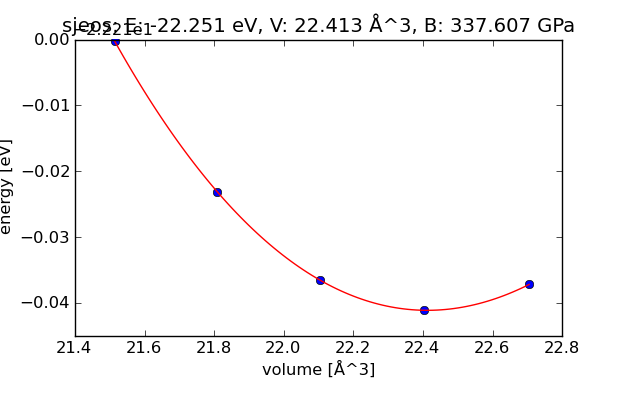
\includegraphics[width=0.7\textwidth]{./6-1.png}
\caption{The equation of state of TaC}
\end{figure}

These results show that the DFT calculated lattice constant of 4.476 \AA{} is higher than the experimental value of 4.455 \AA{}. DFT's calculated bulk modulus of 3.371 Mbar is also lower than 3.45 Mbar.  
\section{Estimate the formation energy of TaC.}
\label{sec-7}

Compute the formation energy of TaC for the reaction Ta + C$_{\mathrm{graphite}}$ $\rightarrow$ TaC. Compare your anser to the value reported in \href{http://pubs.acs.org/doi/pdf/10.1021/j100786a027}{http://pubs.acs.org/doi/pdf/10.1021/j100786a027}. Discuss any reasons for discrepancy. Remember that you must use the same ENCUT for all the calculations in this problem, and you must use the largest ENCUT for all calculations that ensures the accuracy level you want.
\bigskip

To do this calculation, we need total energies at equilibrium volumes at 450 eV kinetic energy cutoff -- 450 eV being the converged energy of graphite. Note that these calculations for graphite and TaC have already been done, since we used VASP to automatically relax the structure. We will however need to do a calculation of Ta at the equilibrium volume calculated by the EOS.


\begin{minted}[frame=lines,fontsize=\scriptsize,linenos]{python}
import sys
from jasp import *

ready = True

# Ta total energy at the equilibrium volume
a = 3.305
a1 = np.array((-a/2, a/2, a/2))
a2 = np.array((a/2, -a/2, a/2))
a3 = np.array((a/2, a/2, -a/2))
Ta = Atoms([Atom('Ta', (0, 0, 0), magmom=6)],
           cell=(a1, a2, a3))
with jasp('7.1/Ta/', atoms=Ta,
          xc='PBE', lreal=False, istart=0,
          encut=450, prec='Accurate',
          kpts=(6, 6, 6), ismear=1, sigma=0.05,
          ispin=2, lorbit=11) as calc:
    try:
        e_Ta = Ta.get_potential_energy()
    except (VaspSubmitted, VaspQueued, VaspRunning):
        ready = False
        pass 

# Graphite total energy at the equilibrium volume
with jasp('5.1/trial1') as calc:
    graphite = calc.get_atoms()
    e_graphite = graphite.get_potential_energy()
    e_graphite = e_graphite / 4 # Since this contains 4 units

# TaC total energy at equilibrium volume
a = 4.476
a1 = np.array((0, a/2, a/2))
a2 = np.array((a/2, 0, a/2))
a3 = np.array((a/2, a/2, 0))
TaC = Atoms([Atom('Ta', (0, 0, 0), magmom=6),
             Atom('C', a1/2 + a2/2 + a3/2, magmom=2)],
            cell=(a1, a2, a3))
with jasp('7.1/TaC',
          xc='PBE', lreal=False, istart=0,
          encut=450, prec='Accurate',
          kpts=(8, 8, 8), ismear=1, sigma=0.05,
          ispin=2, lorbit=11,
          atoms=TaC) as calc:
    try:
        e_TaC = TaC.get_potential_energy()
    except (VaspSubmitted, VaspQueued, VaspRunning):
        ready = False
        pass

# We can now compute the reaction energy for the reaction
e_rxn = e_TaC - e_Ta - e_graphite
print 'The computed enthalpy of the reaction Ta + C -> TaC is {0:1.3f} eV/atom'.format(e_rxn)
print 'Converted to kcal/mol, this is then {0:1.3f} kcal/mol'.format(e_rxn * 23.069)
\end{minted}

\begin{verbatim}
 The compute enthalpy of the reaction Ta + C -> TaC is -1.153 eV/atom
 Converted to kcal/mol, this is then -26.598 kcal/mol
\end{verbatim}

From the article, they reported a formation enthalpy at room temperature of -34.5 \textpm{} 0.9 kcal/mol. Our value is off by about 10 kcal/mol. This shows there is insufficient cancellation error when comparing BCC Ta, graphite C, and rocksalt TaC. This isn't surprising considering how dissimilar the three systems are. We have a metal, a mineral held together by Van der Waals interactions that are not acounted for, and a compound with potential charge transfer and covalent bonding between a metal and a non-metal.

\end{document}
